\documentclass[titlepage, 10pt]{article}

\usepackage{graphicx} %[pdftex]
\usepackage[hidelinks]{hyperref}
\usepackage{titlepic}
\usepackage{amsmath}
\usepackage{fullpage}

\titlepic{
\includegraphics[width=0.30\textwidth]{img/sedes.jpg}}
\title
{
	[H03H1A] Musculoskeletal Biomechanics\\
	Assignment 2: Biomechanical (over-)loading
}
\author{Kim Nuyts \and Sven Van Hove}
\date{\today}

\begin{document}

\pagenumbering{roman} %i, ii, iii
\maketitle

\clearpage
\pagenumbering{Roman} %I, II, III
\tableofcontents

% paragraph makeup, after ToC
\setlength{\parindent}{0pt} %don't indent new paragraph
\setlength{\parskip}{2ex} %add blank line in between

\clearpage
\pagenumbering{arabic} %1, 2, 3

\section{Situation}
\label{sec:intro}
A man is driving a SUV in the village center when suddenly a pedestrian crosses
the road. The man immediately brakes but unfortunately he is unable to stop the
car before it hits the pedestrian. On the bumper of the car a bull bar is
mounted (\autoref{fig:bullbar}) which, in first instance, hits the upper leg of
the pedestrian. In this paper we will investigate what the forces exerted on the
femur by the bull bar are, what the internal stresses in the femur are and
whether the femur will break or not.

\begin{figure}[htp]
\begin{center}
  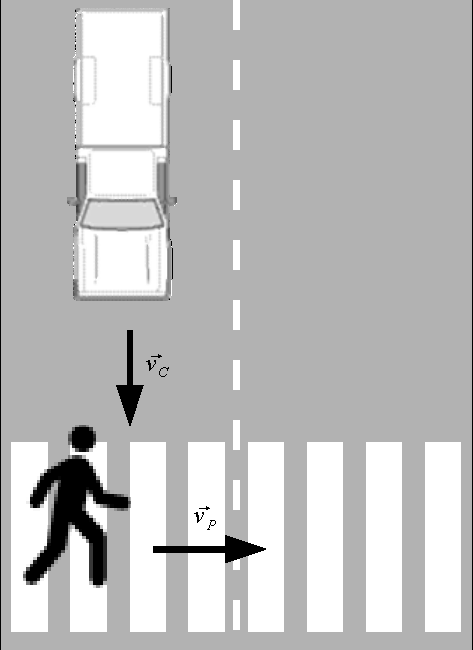
\includegraphics{img/situation.pdf}
  \caption{Overview of the situation.}
  \label{fig:situation}
\end{center}
\end{figure}

In \autoref{fig:events} the initial events in a car-pedestrian collision are
visualized. Although the pictures give the reader a good impression of what
happens during a crash, it is not entirely conforming to the situation
described above. In \autoref{fig:events} a normal passenger car hits the
person in front of it. The bumper of a passenger car is at a much lower height
than the bumper of a SUV. Also, there is no bull bar present.

\begin{figure}[htp]
\begin{center}
  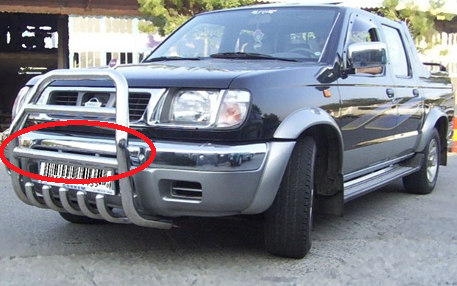
\includegraphics{img/bullbar.png}
  \caption{A bullbar mounted on a car. The protuding part is circled in red.}
  \label{fig:bullbar}
\end{center}
\end{figure}

\begin{figure}[htp]
\begin{center}
  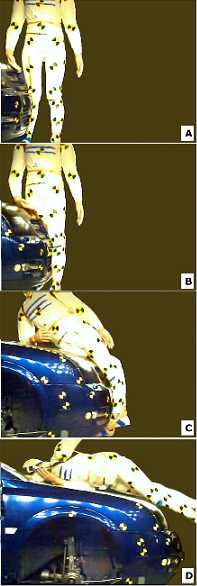
\includegraphics{img/first_instance.png}
  \caption{Subsequent events in car-pedestrian collision.}
  \label{fig:events}
\end{center}
\end{figure}

Now that the situation is properly defined, we will discuss the
assumptions we made in the next section. These will be the basis of our
mechanical analysis in \autoref{sec:analysis}

\section{Assumptions}
\label{sec:assumptions}
\autoref{fig:events} shows how complex even the initial events during a
collision are. As it would be too difficult to analyse these subsequent
situations without the proper software, only the first event (A) is
taken into account to reduce the complexity. To decrease the complexity even
more, a number of assumptions are made. In the following paragraphs these
assumptions are explained in detail.

Our victim is a healthy thirty year old male with a height of 1,80m and a mass
of 80kg. Using \autoref{fig:proportions}, we estimate the distance from
respectively the angle, knee and hip to the ground to be 0,07m, 0,51m and 0,95m.
The lower legs has a mass of 3,72kg and the upper legs has a mass of
8kg\cite{Ob}. The car weighs 2400kg,  the bull bar is made of 
aluminium ($E_{Al}$=69 GPa and $\nu_{Al}$=0,32)
%stainless steel ($E_{SS}$=210 GPa and $\nu_{SS}$=0,305
%\footnote{\url{http://www.engineeringtoolbox.com/poissons-ratio-d_1224.html}})
and its most protuding part sits at 0,80m heigh. \cite{huiskes1977geometrical}
suggest $E_{femur}$ = 20 GPa and $\nu_{femur}$ = 0,37.

%TODO which of these are actually used?
\begin{figure}[htp]
\begin{center}
  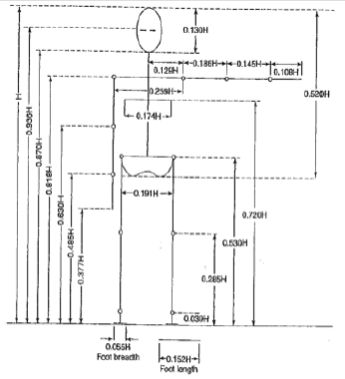
\includegraphics{img/proportions.png}
  \caption{Various lengths of human body segments in proportion to
  total height.}
  \label{fig:proportions}
\end{center}
\end{figure}

Right before the collision the pedestrian is located right in front of the car.
He is walking and at the moment of the crash the leg closest to the car is in
stand phase. The other leg is in swing phase. We examine the femur of the former
leg, because it is most likely to fail. The weight of both his upper and lower
leg segments are also calculated. It is assumed the weight is equally
distributed over the length of both parts, so the center of gravity is situated
in the middle of both parts.

At the time of collision the car is decelerating, but it still has a speed of 36
km/h (10 m/s). Due to the bullbar that is mounted on the bumper, the initial
contact between the body of the pedestrian and the car is limited to the bar of
the bar touching the upper leg of the pedestrian. The femur is the long
bone that provides support in the upper leg. Around the femur the hamstring
muscles, the quadriceps muscles and a layer of fat act as a shock absorbers
during the impact. The literature suggests using a damping factor of roughly
15\% \cite{kannus1999comparison}. %TODO use damping factor

As only the initial phase of the impact is considered in this paper, it is
assumed that the horizontal velocity of the hip is zero at the time of impact .
The foot also remains in place, but rotates inwards at the ankle. Because of
this the bones in the lower leg do not deform. Further it is assumed that the
knee does not bend initially. So the deformation induced by the bull bar is only
reflected in the femur shaft. In reality the knee will also be affected by the
forces exerted by the bull bar. Depending on the situation and the relative strength of
both, the femur will break or the knee will be distorted. In the following
analysis however, it is assumed that the femur will absorb the initial impact.
This means we assume that the knee will not become distorted (so it will
continue to properly connect the upper and lower leg) and that the other bones
�-- from pelvis to the little bones in the foot --� are not affected initially.
Because of these (rather rough) assumptions the whole leg can be treated as one
structure which is clamped at the top (pelvis) and with a hinge at the level of
the ankle. The force exerted on this structure by the bull bar is treated as a
force concentrated in one point at a height of 85 cm. It is assumed that the
bull bar will not deform during the collision, nor that the crumple zone of the
car is activated. %TODO 85 ipv 80?

As the pedestrian is a young male it is assumed he has normal bones, not
affected by any disease. The femoral bone has an average length of 48 cm, a
shaft diameter of 2.43 cm and the femoral canal has a diameter of 13
mm.\footnote{http://www.orthopaedicsone.com}


\section{Mechanical Analysis}
\label{sec:analysis}
In the following paragraphs the effects of the impact of the car on the femur of
the pedestrian are investigated. First an estimation of the forces exerted on
the femur is made. Then a force diagram and bending moment diagrams are calculated.
Based on these diagrams the stresses in the bone are estimated and by comparing
the stresses with experimental data of previous research the probability that
the bone will fail is estimated.

\subsection{Calculating impact force}
We start from the conservation of momentum law in the direction the car is
traveling. This assumes a perfect ellastic collision, which is a very
crude approximation of reality. Because the velocity of the pedestrian in this
direction is zero, so is his momentum. \autoref{fig:events} shows that the car
and the pedestrian cling together during the first few seconds after time of impact, so
we consider them as one system with one momentum.
\begin{equation}
	p_{C_0} + 0 = p_1
\end{equation}

% \begin{equation}
% 	\frac{m_C \cdot v_{C_0}^2}{2} + \frac{m_P \cdot v_{P_0}^2}{2}  = 
% 	\frac{m_C \cdot v_{C_1}^2}{2} + \frac{m_P \cdot v_{P_1}^2}{2}
% \end{equation}

\begin{equation}
	m_C \cdot v_{C_0} + 0 = (m_C + m_P) \cdot v_1
\end{equation}

Solve for $v_1$.
\begin{equation}
	v_1 = \frac{m_C}{m_C + m_P} \cdot v_{C_0} 
	= \frac{2400\text{ kg}}{2480\text{ kg}} \cdot 10 \text{ m/s}
	\approx 9.68 \text{ m/s}
\end{equation}

From this, we can calculate the force acting on the pedestrian.
\begin{equation}
	F' = \frac{\Delta p}{\Delta t}
\end{equation}

The equation shows that the force $F$ is also dependent on the time interval
$\Delta t$ in which the collision occurs. When two hard materials hit each
other, e.g. a club hitting a golfbal, this interval is approximately $400 \mu
s$\footnote{http://www.golfswing.com.au/139}. On the other hand, the typical
impact time - from full speed to standstill - of a car crashing into a wall is
about 100ms \cite{crash_mech}
\footnote{http://auto.howstuffworks.com/car-driving-safety/accidents-hazardous-conditions/crash-test.htm}.
This interval is larger because of crumple zones. However, because our car is
equipped with a bullbar, and because we only take into account the initial
event, we estimate $\Delta t \approx 10$ms.

Plugging this value into the equation gives:
\begin{equation}
	F' = \frac{80\text{ kg} \cdot 9.68\text{ m/s}}{0.01\text{ s}} = 77440\text{ N}
\end{equation}

We assumed a soft tissue damping factor of roughly 15\%, which allows us to
calculate the resulting foce on the femur:
\begin{equation}
	F = 0.85F' = 65824\text{ N}
\end{equation}

\subsection{Discussion on force and bending moment diagrams} 
After the mechanical system in \autoref{sec:assumptions} was decided upon, the
force and bending moment equilibrium equations were calculated in the y-direction.

\begin{equation}
	\Sigma F = 0: R_{Ay} + R_{By} - F = 0
\end{equation}

\begin{equation}
	\Sigma M_z \stackrel{w.r.t. B}{=} 0: L_2 F - (L_1 + L_2)R_{Ay} - M_A = 0 
\end{equation}

We did not calculate the forces in the x-direction, as these were less
relevant for our analysis.

From these equations it is clear we have a hyperstatic sytem of level 1, which
means we have three unknowns and only two equations. Therefore, this system has
to be solved using �the method of the chord�. The first step in applying this
technique is choosing two points $a$ and $b$ that are fixed in your system. Then
a point $c$ is determined which is situated between points $a$ and $b$. Point
$c$ indicates where you want to calculate the deformation in the
system due to external forces and bending moments. In this case point $c$ coincides with point $a$. Next the bending moment
diagram $M$, taking into account all external forces, is calculated. From this
bending moment diagram $M$ the reduced bending moment $M_{red}$ is deduced by dividing M by the
multiplication of the Young�s modulus and the moment of inertia of the system
($EI$). In this way the stiffness of the system is also taken into account. This
allows us to get an exact solution for the hyperstatic mechanical system.


In the next step the reduced bending moment diagram is treated as a
distributed force acting on the entire length of the beams. To calculate the equivalent force of these
distributed forces the reduced bending moment diagram is divided into triangular
parts. For each of these triangular parts an $F_{eq}$ is calculated. By
applying a force and bending moment equilibrium on each part of the beam the
reaction force in point $c$ is determined.
The method of the chord then states that the reaction force in this point
is equal to the angle of deformation in that point.

In order to solve the hyperstatic system it has to be divided into two
subsystems: a main system (\autoref{fig:hyper2main}) and a recovery system
(\autoref{fig:hyper3recovery}). The main system is the hyperstatic system made
static again by cancelling one force or bending moment. In this case we chose to cancel
the bending moment of the clamped pelvis. The task of the recovery system is to restore
the distortion, due to cancelling the bending moment, of the line of deformation
of the main system. Therefore, a bending moment $m_a$ is added in the
recovery system. The method of the chord is applied on both systems and then the
results of the two systems are superimposed to obtain the results for the
initial hyperstatic system.

 \begin{figure}[htp]
\begin{center}
  \includegraphics[page=2,width=\textwidth]{img/hyper.pdf}
  \caption{The main system (HS).}
  \label{fig:hyper2main}
\end{center}
\end{figure}

\begin{figure}[htp]
\begin{center}
  \includegraphics[page=3,width=\textwidth]{img/hyper.pdf}
  \caption{The recovery system (hs).}
  \label{fig:hyper3recovery}
\end{center}
\end{figure}

\subsubsection{Analysis of the main system}
First, we calculate the bending moment $M$ for the main system. From this
bending moment $M$ the reduced bending moment $M_{red}$ is deduced in
\autoref{fig:hyper4}.

\begin{equation}
	M_{HS} = R_A \cdot L_1 = \frac{-L_1 \cdot L_2}{L_1 + L_2} \cdot F
\end{equation}

\begin{equation}
	M_{red} = \frac{-L_1 \cdot L_2}{L_1 + L_2} \cdot \frac{F}{EI}
\end{equation}

Based on $M_{red}$ the equivalent forces $F_e$ are calculated. Then $R_A$ (and
thus $\theta_{HS}$) is calculated.

\begin{equation}
	F_{e_1} = \frac{-L_1 L_2}{L_1+ L_2} \frac{F}{EI} \frac{L_1}{2}
\end{equation}

\begin{equation}
	F_{e_2} = \frac{-L_1 L_2}{L_1+ L_2} \frac{F}{EI} \frac{L_2}{2}
\end{equation}

\begin{equation}
	\Sigma M_z \stackrel{w.r.t. b}{=} 0: \frac{2}{3} L_2 F_{e_2} + (L_2 +
	\frac{1}{3}L_1) F_{e_1} - R_A (L_1 + L_2) = 0
\end{equation}

\begin{equation}\label{eq:RA}
	R_A = \frac{\frac{2}{3} L_2 F_{e_2} + L_2 F_{e_1} + \frac{1}{3}L_1 F_{e_1}}{L_1 +
	L_2} = \theta_{HS}
\end{equation}

\begin{equation}
	R_A = \frac{-1}{3} \frac{L_1 L_2^3 F}{(L_1 + L_2)^2 EI} - \frac{L_1^2 L_2^2
	F}{(L_1 + L_2)^2 2EI} - \frac{-1}{6} \frac{L_1^3 L_2 F}{(L_1 + L_2)^2 EI} =
	\theta_{HS}
\end{equation}

\begin{figure}[htp]
\begin{center}
  \includegraphics[page=4,width=\textwidth]{img/hyper.pdf}
  \caption{Reduced bending moment diagram $M_{red}$ of the main system.}
  \label{fig:hyper4}
\end{center}
\end{figure}

\subsubsection{Analysis of the recovery system}
We repeat this exercise for the recovery system in \autoref{fig:hyper5}.
\begin{equation}
	M_{hs} = -m = -m_a
\end{equation}

\begin{equation}
	M_{red} = \frac{-m}{EI}
\end{equation}

\begin{equation}
	\Sigma M_z \stackrel{w.r.t. b}{=} 0: \frac{2}{3}(L_1 + L_2)F_e - (L_1+L_2) R_a = 0
\end{equation}

Solve for $R_a$:
\begin{equation}
	R_a = \frac{\frac{2}{3}(L_1 + L_2)F_e}{L_1 + L_2} = \frac{2}{3} F_e
\end{equation}

We also know $F_e$:
\begin{equation}
	F_e = \frac{-m}{EI} \frac{L_1 + L_2}{2}
\end{equation}

So we can rewrite $R_a$ as:
\begin{equation}
	R_a = \frac{-2}{3} \frac{m}{EI} \frac{L_1 + L_2}{2} = \theta_{hs}
\end{equation}

\begin{figure}[htp]
\begin{center}
  \includegraphics[page=5,width=\textwidth]{img/hyper.pdf}
  \caption{Reduced bending moment diagram of the recovery system.}
  \label{fig:hyper5}
\end{center}
\end{figure}

\subsubsection{Combining both systems}
To combine the two systems, the following equation must hold:
\begin{equation}
	\theta_{HS} + \theta_{hs} = 0
\end{equation}

\begin{equation}
	\frac{-1}{3} \frac{L_1 L_2^3 F}{(L_1 + L_2)^2 EI} - \frac{L_1^2 L_2^2
	F}{(L_1 + L_2)^2 2EI} - \frac{1}{6} \frac{L_1^3 L_2 F}{(L_1 + L_2)^2 EI} -
	\frac{2}{3} \frac{m}{EI} \frac{L_1 + L_2}{2} = 0
\end{equation}

Solve for m:
\begin{equation}
	m = \frac{-2 L_1 L_2^3F - 3 L_1^2 L_2^2 - L_1^3 L_2 F}{2(L_1 + L_2)^3}
\end{equation}

Using $L_1 = 0.154$m, $L_2 = 0.8$m and $F = 65824$N, we can calculate $M_A$ by
applying the superposition principle in point $c$:
\begin{equation}
	M_A = 0-m = 7814.44\text{Nm}
\end{equation}

\subsubsection{Solving the original system}
With this knowledge, we can finally solve the original system and construct the
accompanying force (\autoref{fig:hyper6}) and bending moment (\autoref{fig:hyper7})
diagrams by using the principle of superposition.

\begin{equation}
	R_{Ay} = \frac{L_2}{L_1 + L_2} F = 55 198.32 \text{N}
\end{equation}

\begin{equation}
	R_{By} = \frac{L_1}{L_1 + L_2} F = 10 625.68 \text{N}
\end{equation}

\begin{equation}
	M_A = 7814.44\text{Nm}
\end{equation}

\begin{equation}
	 M_{HS_{at force F}} = - \frac{L_1 L_2}{L_1 + L_2} F = - 8 500.54 \text{Nm}
\end{equation}

\begin{equation}
	 M_{hs_{at force F}} = \frac{L_2 M_A}{L_1 + L_2} = 6 552.98 \text{Nm}
\end{equation}

\begin{equation}
	 M_{at force F} = M_{HS_{at force F}} + M_{hs_{at force F}} = - 1947,56
	 \text{Nm}
\end{equation}

\begin{figure}[htp]
\begin{center}
  \includegraphics[page=6,width=\textwidth]{img/hyper.pdf}
  \caption{Force diagram of the original system.}
  \label{fig:hyper6}
\end{center}
\end{figure}

\begin{figure}[htp]
\begin{center}
  \includegraphics[page=7,width=\textwidth]{img/hyper.pdf}
  \caption{Bending moment diagram of the original system.}
  \label{fig:hyper7}
\end{center}
\end{figure}

The forces applied on the upper part of the upper leg are definitely the
largest: they are five times larger than the forces applied on the lower parts.
Nevertheless, both distributed forces are of significant magnitude: 55,2 kN  and
10,6 kN. As they are exerted in the transverse direction on the femur, it is
very likely they will cause a fracture of the bone. All long bones have
anisotropic structure characteristics. This causes them to be weaker in the
transverse direction than in the longitudinal direction, which makes a fracture
in our scenario very likely.

\subsection{Calculating stress in the femur}
In this section, we calculate the stress $\sigma$ in the femur, assuming it
has not yet broken. For this, we need the applied force $F$ and the contact area
$A$. We already know $F$, so this section will focus on estimating $A$. To do
so, we make use of Hertz theory. We model both the femur and the bull bar as
cylinders, and assume they are in direct contact. This theory requires three
main assumptions to hold true:
\begin{enumerate}
  \item both materials must have a similar Young's modulus
  \item both surfaces must deform
  \item the contact area must be relatively small compared to the two bodies in
  contact
\end{enumerate}

The first assumption will hold true in our case because the Young's modulus of
the femur bone is 20 GPa and of the aluminium bull bar is 69 GPa, which is only
a factor 3.5 difference. For the second assumption we can expect that the
deformation will mostly affect the femur rather than the bull bar. The third
assumption is likely to be met as well.

Out goal is to calculate the area $A$ of the circular contact area. This
requires a contact radius $a$:
\begin{equation}
	a = \sqrt{Rd}
\end{equation}

We estimate the radius of the femur and bull bar as respectively $R_{bone} =
12.15$mm and $R_{bar} = 30.00$mm. The diameters $D_{bone}$ and $D_{bar}$ are
obviously double those values. Combining these two radii with the
formule below yields $R$:
\begin{equation}
	\frac{1}{R} = \frac{1}{R_{bone}} + \frac{1}{R_{bar}} = 115.3 \text{1/m} \Leftrightarrow R = 0.0087\text{m} 
\end{equation}

We can also calculate $d$ -- the total elastic compression at the contact
surface, measured along the line of the applied force $F$ -- using a formule
proposed by \cite{puttock1969elastic}:

\begin{equation}
	d = \frac{(3\pi)^\frac{2}{3}}{2} \cdot F^\frac{2}{3} \cdot (v_{bone} +
	v_{bar})^\frac{2}{3} \cdot \left(\frac{1}{D_{bone}}\right)^\frac{1}{3}
\end{equation}

Herein, $\nu_{bone}$ and $\nu_{bar}$ are given by:
\begin{equation}
	v_{bone} = \frac{1 - \nu_{femur}^2}{\pi E_{femur}} = \frac{1 - 0,37^2}{\pi
	\cdot 20\text{ GPa}} = 1,3737 \cdot 10^{-11} \frac{1}{\text{Pa}}
\end{equation}
\begin{equation}
	v_{bar} = \frac{1 - \nu_{Al}^2}{\pi E_{Al}} = \frac{1 - 0.32^2}{\pi \cdot
	69\text{ GPa}} = 4.1408 \cdot 10^{-12} \frac{1}{\text{Pa}}
\end{equation}

Plug in all known variables, and we get this result:
\begin{equation}
	d = \frac{(3\pi)^\frac{2}{3}}{2} \cdot (65824\text{ N})^\frac{2}{3} \cdot
	(1,3737 \cdot 10^{-11} \frac{1}{\text{Pa}} + 4,1408 \cdot 10^{-12}
	\frac{1}{\text{Pa}})^\frac{2}{3} \cdot \left(\frac{1}{0,0243\text{
	m}}\right)^\frac{1}{3} = 0,0008585\text{ m}
\end{equation}

At last, we can find $A$ and thus $\sigma$:
\begin{equation}
	A = \pi  a^2 = \pi R d = 0,000023465 \text{ m}^2
\end{equation}

\begin{equation}
	\sigma = \frac{F}{A} = \frac{65824\text{ N}}{0,000023465 \text{ m}^2} = 28052
	\cdot 10^5\text{ Pa} \approx 2,8\text{ GPa}
\end{equation}

\subsection{Will the femur break?}

According to our calculations above, the transverse stresses at the contact
area are approximately 2,8 GPa. We compare this with the values in table
\autoref{fig:femurprop}. As 2,8 GPa is much higher than 133 MPa, the maximum
compression stresses are exceeded, and thus the femur will break. Note that we
made no distinction between cortical and trabecular bone. Because the table
only contains data for the relatively stronger cortical bone, it is safe to
assume that it will fracture regardless. 

As soon as the femur fractures, it can no longer absorb the stresses.
Instead, they are redirected to the soft tissue. However, the damage
calculations in this case are out of the scope of this report.

%TODO: F is linear in speed. Reaction forces and torques are linear in F.
% -> easy to calculate maximum speed so that femur won't break? 

\begin{figure}[htp]
\begin{center}
  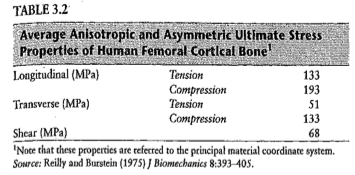
\includegraphics{img/properties_femur.png}
  \caption{Properties of the femur. \cite{Ob}}
  \label{fig:femurprop}
\end{center}
\end{figure}


\section{Conclusion}
CT technology has come to the point where high resolution images of the whole
chest can be obtained in a single breath hold. The resolution allows to detect
pulmonary nodules in an early stage and therefore CT scans become more and more
part of routine investigations. This causes a large increase in the workload of
the radiologists, who are only human and thus also prone to errors. Time
pressure and fatigue may lead to an increasing fraction of overlooked nodules.
Research showed however that pulmonary lung detection systems, that serve as a
second reader, can improve the performances of radiologists.
Therefore, the goal of this project was to develop an accurate, fast and
automated system to detect pulmonary nodules in CT scans.

A non-exhaustive literature review revealed that companies such as R2
Technology, Siemens, iCAD etc. already have invested in the development of
similar software. However, a satisfying allround software package does not exist
yet. The research is still ongoing to develop a system with 100\% sensitivity
and no false positives detection. One of the problems that arises here is that
there is no golden standard to measure the performance of the CAD system
against. Currently, the performances of CAD systems are compared with the
findings of one or more radiologists. Although the fraction of overlooked
nodules decreases when more radiologists cooperate when analysing a CT scan,
there is no guarantee that all nodules are delineated in a scan. This makes it
very hard to assess the performance of a automated nodule detection system.

There are three main schools of thought in the development of pulmonary nodule CAD
systems. The first group uses template matching to detect (a type of) nodules. A
second group performs a nodule segmentation by means of a series of
morphological operations, active contour modelling, etc. The third group applies
classification methods, possibly aided by clustering. As there is evidence
in literature that this method yields the best results, a more extensive
literature review was performed to select a proper classification method. It was
decided to use a cascaded Random Forest classifier as this type of classifiers
is not yet fully explored in this area of research. This provided the
opportunity to beat the state of the art in nodule detection algorithms.

Random Forests have many advantages. As an ensemble classifier it combines
decisions of multiple classifiers to form an integrated output. This way of
working has the advantage that a better predictive performance is obtained
compared to the predictive performance demonstrated by each individual learning
algorithm separately. Furthermore, Random Forests are rather robust against
noise compared with other classifier such as Support Vector Machines. Random
Forests also allow to use a lot of features, even if they have different orders
of magnitude, without increasing the time complexity too much. The features also
do not have to be known in advance. At the same time, the method does not
require a lot of parameter tuning. The only thing that has to be taken into
consideration is the depth of the trees as overfitting must be avoided in order
to maintain an algorithm that is able to generalise across datasets. The use of
a cascaded classifier is preferred as it limits the amount of CPU time and
memory storage.
 
The higher the level in the cascaded classifier, the more complex the features.
On the first level the grey values of the voxels were used to detect soft
tissue, to which class nodules belong. Although this first level is able to
eliminate the voxels outside the lungs, a lung segmentation was applied first to
reduce the amount of voxels to be processed. The reason for this were recurrent
memory errors when attempted otherwise. On the second level a blobdetector --
Laplacian filter -- and a distance map were implemented. On the third and fourth
level a 3D averaging algorithm was elaborated with two different
parametersettings. This 3D averaging allows to separate nodules from bronchioles
and bronchi by taking into account the presence of these structures in the
preceeding and/or succeeding slices. A lot of other features were implemented
and tested, but most of them were removed again from the final classifier as
they required a lot of processing time and did not perform accordingly. After
each level in the classifier a threshold was set to determine which voxels were
taken to the next level and which were to be discarded. These thresholds were
empirically determined, but can still be optimised. The training and the
validation of the algorithm were performed on 30 and 8 datasets respectively.

During the training of the algorithm a five-fold crossvalidation was performed
to determine the optimal set of parameters for the Random Forest algorithm. It
was decided to take into account the optimal number of minimum samples per leaf
to keep the algorithm from overfitting. An accuracy level of 98,2\% was achieved
in the last level of the cascaded classifier.

The validation of the optimised classifier showed 100\% sensitivity, but also
indicated the amount of false positives still has to be significantly reduced.
The processing time of 10 minutes per scan is not extremely satisfying, but one
has to take into account that Python is an interpreted language which makes it
inherently slower than for instance C++. Transferring the code to a compiled
language will speed up the process. The aim is to be able to process one scan
within a few minutes. There is no need for faster processing as a radiologist
will not need the results earlier, but it should not take much longer either.

The amount of false positives per scan (4279,43 FP per scan) has to be reduced.
A first step to achieve this is the optimisation of the thresholds in the
algorithm. A more accurate setting of the thresholds will also be possible if the
algorithm is trained on a larger amount of scans. On top of that, the clustering
strategy might have to be revisited. Another possibility is the implementation
of more features. However, there are two constraints here. The first
one is trivial: the more features, the longer it will take to process the scan.
A second consideration that has to be made is the fact that not all features are
suitable for our approach. We only selected features that could be extracted
from the image without performing any nodule segmentation in advance to make the
algorithm faster an more robust. This nodule segmentation step would allow to
use a wider range of features, but could also introduce errors in the algorithm.
Furthermore, developing a nodule segmentation is not a trivial thing to do.

Although the use of the features and the code of the cascaded classifier were
optimised considerably, one of the largest problems we encountered were the
recurring out-of-memory errors. In the beginning of the project we decided to
use Python 2.7.6 in the 32-bit version as it is typically more stable than the
64-bit version. This showed to be a bad choice later on as we had to spend a lot
of time and efforts on the optimisation of the code concerning memory storage
and computational power. This also prevented us from implementing a lot of
features as we intended to do. The first concept was to calculate a range of
features and let the Random Forest algorithm then decide on which and how many
features to use in the final classifier. Because of the memory errors, we had to
carefully select the features ourselves by visual assessment of the probability
images that were generated at each level in the classifier, rather than letting
RF figure out the most interesting features from a large pool.

Some other things to be done differently in the future is limiting the amount
of time spent on reviewing the literature, limiting the amount of time spent
on optimising the threshold values and performing the implementation of the
features in a different way. In the beginning of the project we implemented a
lot of features, which was also the aim before we encountered the memory
errors, but a lot of them proved to be useless or required too much processing
time. Instead, we should have tried some features, trained the algorithm and
make decisions on the type and amount of feautures based on these small
experiments.

Besides the suggestions for improvement mentioned above, we have some other
recommendations for future research. First of all, it would be interesting to
not only detect the nodules, but also classify them as benign or malignant. In
order to do this the grey value intensity gradient inside the nodule could be a
helpful feature. In order to implement this feature, the nodule voxels should be
clustered first. Also classifying the nodules accoring to the type of nodule
(juxta-vascular; pleural tail; well-circumscribed; juxta-pleural) would be
interesing as the type may already be an indication for the probability of
malignancy of a nodule. As the type of nodule was not available in the
annotations, it was not possible for us to implement this in the classifier.
An interesting comparison that can be made is whether the subtelty
that is assigned by the radiologist is comparible with the probability provided
by the algorithm. And may the algorithm overlook the same nodules as one
radiologist when assessing the CT scan?

Finally, if all optimalisations are performed the algorithm can be implemented
in MeVisLab as a stand-alone modules which can easily be used by radiologists or
researchers. To assess the performance of the optimised algorithm it can be
validated on the dataset of the ANODE09 challenge where it can be compared with
the results of other studies.

\bibliographystyle{alpha} %plain,unsrt,alpha,abbrv,acm,apalike,siam,ieeetr,..
\bibliography{references}
\end{document}